%license:BSD-3-Clause
%copyright-holders:Michele Maione
%============================================================
%
%	Piattaforma di cloud gaming per giochi arcade
%
%============================================================

\chapter{Il cloud gaming}
Il capitolo che apre questa tesi fa un'introduzione sulla nascita dei videogiochi, i ricavi globali dell'industria videoludica, il cloud gaming e i servizi presenti sul mercato.




\section{La nascita dei videogiochi}
Nel 1952 nei laboratori dell'Università di Cambridge, come esempio a corredo di una tesi di dottorato sull'interazione uomo-macchina, fu creato OXO, la trasposizione del tris come gioco per computer. OXO è considerato tecnicamente il primo videogioco. Nel 1958 un professore di fisica del Brookhaven National Laboratory creò un gioco, Tennis for Two, che aveva il compito di simulare le leggi fisiche relative ad una partita di tennis, lo strumento utilizzato era un oscilloscopio.

Nel 1961, sei giovani scienziati del Massachusetts Institute of Technology su un PDP-1\footnote{PDP-1: Programmed Data Processor-1, era un computer della Digital Equipment Corporation del 1959.} crearono il primo videogioco a scopo di intrattenimento: Spacewar!.

Due mesi dopo due ingegneri elettrici, N. Bushnell e T. Dabney, terminarono la loro versione di Spacewar! su larga scala (1.500 copie), ma il gioco non ebbe un grande successo a causa dell'elevata difficoltà. Bushnell, dopo l'esperimento non particolarmente riuscito, decise però di insistere nel settore dando così vita alla società Atari. Il primo gioco arcade di Atari fu il primo grande successo del settore: Pong. Pubblicato alla fine del 1972, è un gioco che riproduce approssimativamente la meccanica del ping pong. Atari vendette 19.000 cabinati di Pong e presto molte altre società seguirono l'esempio. Alla fine del decennio iniziò l'epoca d'oro dei videogiochi arcade e la nascita delle console (console che hanno fatto la storia in Fig. \ref{fig:consoles_history}).

\begin{figure}[H]
	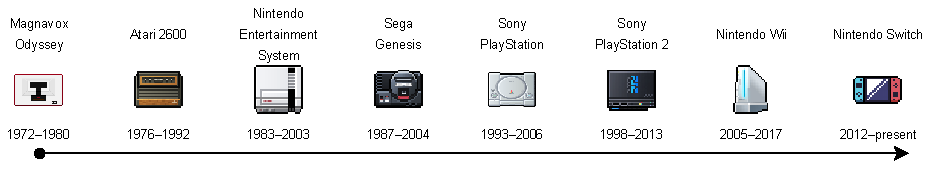
\includegraphics[width=\linewidth]{immagini/consoles_history}
	\caption{Console iconiche, fino alla generazione otto}
	\label{fig:consoles_history}
\end{figure}

I videogiochi sono un mezzo di intrattenimento unico che combina le diverse forme d'arte, quali musica, narrativa e animazione, all'interattività. Ed è proprio questa caratteristica, l'interattività, che permette loro di esercitare un potenziale d'immersione e attrazione che altri media non hanno. Sono ormai diventati un fenomeno culturale di massa con centinaia di milioni di persone che giocano regolarmente ogni giorno, il che li rende un attore dominante nel settore dell'intrattenimento, settore in continua crescita che non ha mai subito interruzioni nel corso degli anni come mostrato in Fig. \ref{fig:valore_commerciale_giochi_globale}. Negli ultimi vent'anni l'importanza economica dei videogiochi arcade è notevolmente diminuita\footnote{Giappone, Cina e Corea mantengono una forte industria arcade ai giorni nostri.} (in viola nella figura) a favore dei videogiochi per personal computer, console e più recentemente per mobile.

\begin{figure}[H]
	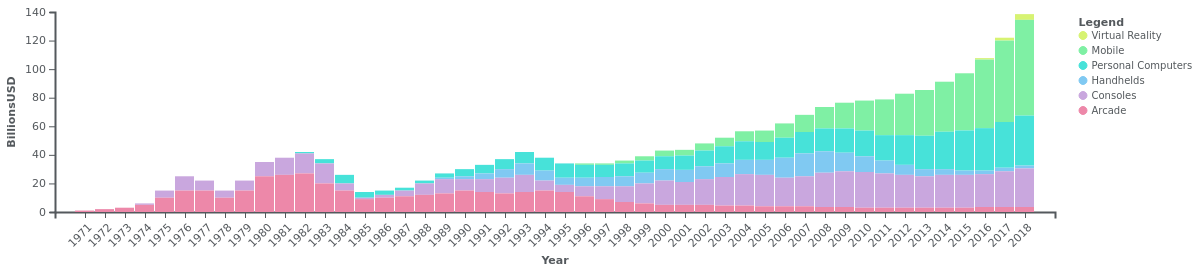
\includegraphics[width=\linewidth]{immagini/valore_commerciale_giochi_globale.png}
	\caption{Ricavi globali dell'industria dei videogiochi dal 1971 al 2018 (non adeguati all'inflazione). Fonte: wikipedia.org}
	\label{fig:valore_commerciale_giochi_globale}
\end{figure}




\section{Cloud gaming}
Il cloud gaming è un servizio che unisce il cloud computing e lo streaming per rendere possibile videogiocare in remoto senza scaricare o installare il gioco sul device dell'utente, in pratica i videogiochi vengono archiviati ed eseguiti su un server remoto e l'output audio-video viene trasmesso in streaming (come un filmato) ad un client sul dispositivo dell'utente. Il client gestisce l'input del giocatore che viene inviato al server ed eseguito nel gioco. Come mostrato in Fig. \ref{fig:cloud_gaming_general_scheme} le fasi di elaborazione input, esecuzione del gioco, rendering e missaggio audio, che solitamente vengono eseguite sul dispositivo del giocatore, nel paradigma del cloud gaming vengono eseguite sul server. Sempre sul server c'è una fase di codifica sotto forma di filmato dell'output audio-video del gioco ed invio tramite rete. Sul dispositivo dell'utente ci sono solo due fasi: cattura e trasmissione al server dell'input utente e ricezione e decodifica del filmato dal server. In questo modo il dispositivo dell'utente è indipendente sia dall'hardware che dal sistema operativo a patto che il client possa essere eseguito sul dispositivo dell'utente.

\begin{figure}[H]
	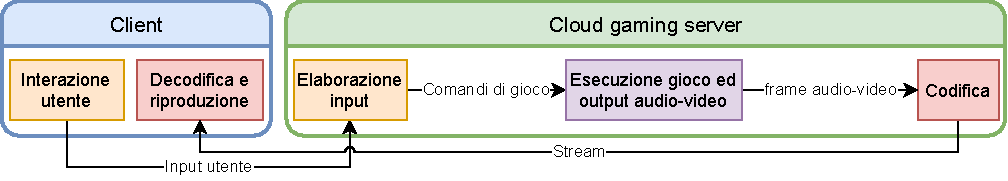
\includegraphics[width=\linewidth]{immagini/cloud_gaming_general_scheme}
	\caption{Architettura del cloud gaming}
	\label{fig:cloud_gaming_general_scheme}
\end{figure}

Secondo una ricerca di Newzoo sull'industria dei videogiochi, come mostrato in Fig. \ref{fig:Newzoo_Cloud_Gaming_Revenues}, nel 2020 il mercato del cloud gaming ha generato quasi 584,7 milioni di USD di entrate, di cui il 39\% e il 29\% in Nord America e in Europa, e si prevede una crescita fino a 4,8 miliardi di USD entro il 2023, se non maggiore. Per questo sono entrate nel mercato del cloud gaming anche aziende che non sono editori o produttori di videogiochi, come Google e Amazon, come vedremo nel paragrafo \ref{StoriaDelCloudGaming}. Queste previsioni sono specchio sia di connessioni di rete sempre più veloci sia nelle case degli utenti sia in mobilità, sia del paradigma dello streaming a cui oggi (sopratutto le nuove generazioni) siamo abituati, di poter accedere instantaneamente a canzoni, video clip, serie tv, film e perché no? videogiochi! Dal punto di vista del giocatore il cloud gaming offre molti vantaggi tra cui: rendere il gioco facilmente accessibile senza la necessità di scaricarlo e installarlo localmente; compatibilità con computer, smartphone e anche con smart TV (se utilizzato con un gamepad WiFi) senza dover badare ai requisiti hardware; diverse modalità di pagamento tra cui l'acquisto di un gioco su richiesta e l'abbonamento mensile/annuale per l'utilizzo di tutta (o una parte) della libreria videoludica; funzionalità aggiuntive per sfruttare al meglio questo modello, come lo streaming della sessione di gioco, cosa che siamo già abituati a vedere, ma con l'aggiunta di dare la possibilità ad uno spettatore di entrare a far parte della propria partita, funzionalità avanzate per il multiplayer come la condivisione della visuale di gioco e dei salvataggi di gioco, ecc\dots. Ma i vantaggi ci sono anche per gli sviluppatori perché il cloud gaming riduce i costi di produzione limitando lo sviluppo e il testing ad una sola piattaforma ed inoltre risolve definitivamente un problema che esiste dai tempi delle audiocassette e dei floppy disk, la pirateria. Non ultimi i fornitori di servizi che si ritrovano con un nuovo modello di business disponibile su contenuti già esistenti. Tuttavia bisogna dire che ci sono anche degli svantaggi, di cui parleremo nel capitolo \ref{Capitolo4}: perdita della qualità audio-video a causa della compressione, larghezza di banda richiesta all'utente non soddisfabile e l'ineliminabile latenza.

\begin{figure}[H]
	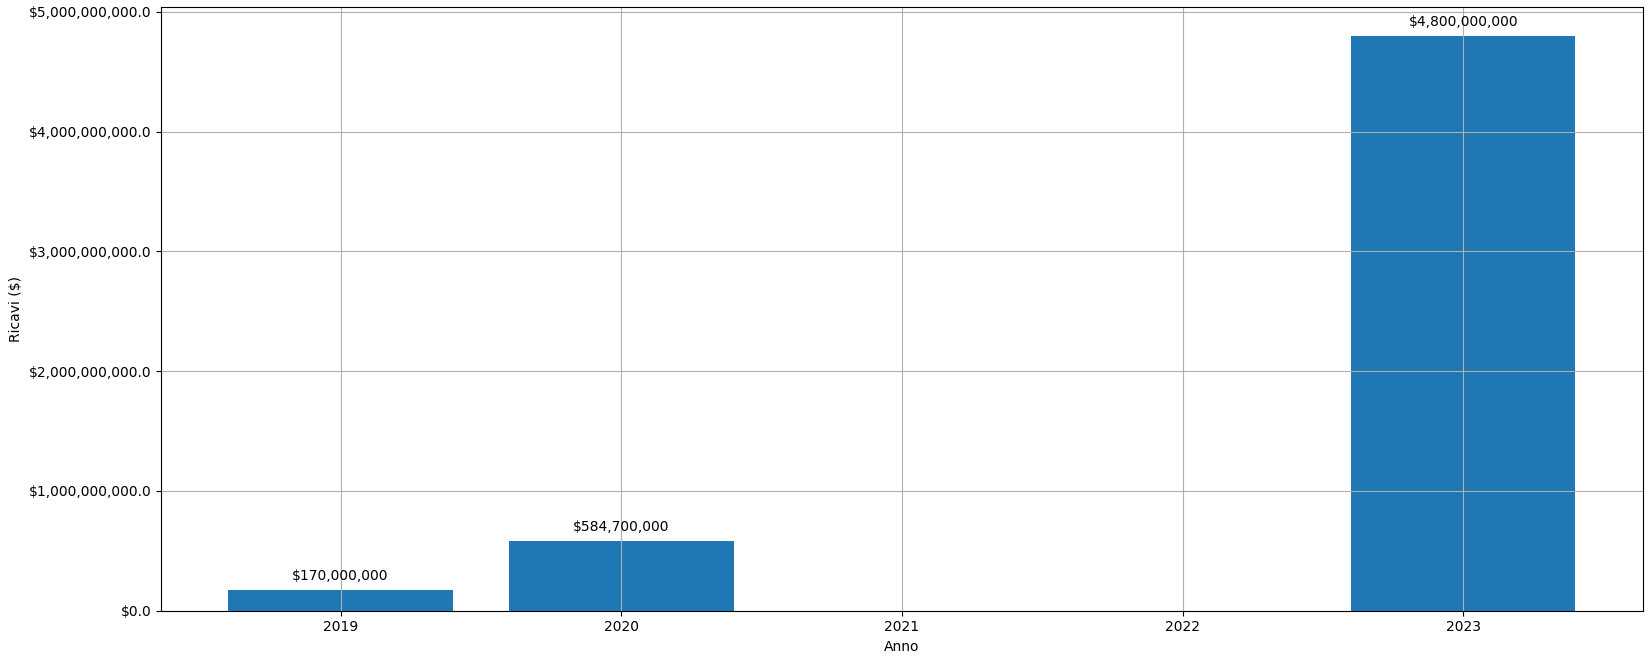
\includegraphics[width=\linewidth]{immagini/Newzoo_Cloud_Gaming_Revenues}
	\caption{Previsioni per il mercato globale del cloud gaming (in dollari americani). Fonte: newzoo.com/global-cloud-gaming-report}
	\label{fig:Newzoo_Cloud_Gaming_Revenues}
\end{figure}



\subsection{Storia del cloud gaming} \label{StoriaDelCloudGaming}
Una delle prime piattaforme di cloud gaming è stata OnLive di OL2, presentato alla GDC\footnote{GDC: Game Developers Conference, una conferenza annuale per gli sviluppatori di videogiochi.} 2009 e poi lanciato sul mercato a giugno 2010 negli Stati Uniti e a settembre 2011 nel Regno Unito. I giocatori, previo pagamento di un abbonamento mensile di 15\$, potevano acquistare o noleggiare giochi sulla piattaforma oppure utilizzare quelli precedentemente acquistati su Steam\footnote{Steam è un servizio di distribuzione digitale di videogiochi della società Valve.}. Il servizio era ospitato su 5 data centers situati sul suolo americano che servivano gli utenti per vicinanza geografica; la qualità video offerta era SD\footnote{Standard definition (SD) include i formati video con rapporto 4:3 e 16:9 con 480 linee di risoluzione (raramente 576).} e HD\footnote{High definition (HD) è un formato video 16:9 con 720 linee di risoluzione.} con una larghezza di banda richiesta di 5 Mbps. Era disponibile, oltre ad un client per Windows, macOS ed Android, anche una micro console da collegare alla TV. Il servizio fu chiuso ad aprile 2015 dopo essere stato acquistato da Sony\cite{Cloud_gaming_history}.

Nel febbraio 2012 Gaikai ha inaugurato il suo omonimo servizio di cloud gaming disponibile in 12 nazioni e distribuito su 24 data centers. La società si è concentrata principalmente sull'utilizzo del cloud gaming come forma di pubblicità online per i videogiochi, dove gli utenti avrebbero avuto la possibilità di accedere alle demo dei videogiochi sponsorizzati. La piattaforma era accessibile tramite browser (utilizzando il plugin di streaming disponibile in Adobe Flash, Java o Google Native Client), la qualità video HD richiedeva una larghezza di banda minima di 5 Mbps. La società fu acquisita da Sony a luglio 2012 per integrare la tecnologia di streaming di Gaikai nella piattaforma di cloud gaming PlayStation Now di Sony\cite{Gaikai_Beta}.

PlayStation Now è un servizio di cloud gaming basato sulla tecnologia cloud di Gaikai. È stato presentato durante il CES\footnote{CES: Consumer Electronics Show, un evento annuale che ospita presentazioni di nuovi prodotti e tecnologie nel settore dell'elettronica di consumo.} 2014. È disponibile da gennaio 2015 in Nord America, da settembre in Giappone e Regno Unito ed ha iniziato ad operare in Europa gradualmente da agosto 2017 a marzo 2019. La piattaforma consente all'utente di giocare ai titoli PlayStation (attualmente dal catalogo giochi della PS2, PS3 e PS4) su PS4, PS5 e Windows\cite{PlayStation_Now}.

La piattaforma Utomik è stata lanciata in beta a giugno 2015 e commercialmente nel maggio 2018 e da allora è in servizio. I giochi per essere riprodotti in un browser richiedono del plug-in Utomik Player. La piattaforma offre un SDK, plug-in e servizi online per creare, avviare, mantenere e monitorare i giochi pubblicati\cite{Utomik}.

GeForce Now è il servizio di cloud gaming di Nvidia lanciato in beta a gennaio 2017 e ufficialmente a febbraio 2020. GeForce Now consente agli utenti di accedere da remoto (tramite streaming) a un computer virtuale, dove possono installare giochi acquistati su Steam, Ubisoft Connect\footnote{Ubisoft Connect è un servizio di distribuzione digitale della società Ubisoft.} o Epic Games Store\footnote{Epic Games Store è un negozio di videogiochi digitali gestito da Epic Games.}. Il servizio può essere utilizzato su Windows, macOS, iOS, Android o Nvidia Shield TV\footnote{Nvidia Shield TV è un lettore multimediale digitale basato su Android.}\cite{GeForce_Now}.

A maggio 2018 Electronic Arts ha svelato la sua piattaforma di cloud gaming chiamata Project Atlas, che mira a rendere disponibili numerosi titoli e a fornire un'esperienza di gioco mai provata prima grazie al supporto dell'intelligenza artificiale. La piattaforma mira ad offrire un'esperienza di gioco composta da universi realmente viventi, che cambiano con il passare del tempo, con l'interazione con altri giocatori e sotto l'influenza del mondo esterno. In questi processi, il supporto dell'intelligenza artificiale e l'apprendimento delle abitudini e delle preferenze dei giocatori giocherebbero un ruolo fondamentale. Offre anche un client di gioco dinamico, che consente agli utenti di riprodurre in streaming un titolo mentre attendono il completamento del download sul proprio dispositivo\cite{Project_Atlas}.

RemoteMyApp della Vortex è un servizio di cloud gaming lanciato a novembre 2018, è disponibile per Android, Windows e macOS e offre tre piani mensili (12\$, 23\$ e 33\$) che consentono all'utente di giocare per un massimo di 140 ore al mese ad un catalogo di 170 giochi. Sfortunatamente, alcuni giochi possono essere riprodotti solo acquistando la licenza del gioco\cite{RemoteMyApp_Vortex}.

Microsoft ha anticipato Xbox Cloud Gaming all'E3\footnote{E3: Electronic Entertainment Expo, un evento commerciale per l'industria dei videogiochi.} 2018. La piattaforma è disponibile per gli abbonati a Xbox Game Pass Ultimate da settembre 2020 ed offre sia la libreria esistente di giochi per Xbox che per Xbox Series X. Il servizio è progettato per funzionare con gli smartphone (attualmente solo Android), con controlli touchscreen o usando un controller Xbox tramite Bluetooth\cite{Xbox_Game_Pass_cloud_gaming}.

Google Stadia è una piattaforma di cloud gaming rilasciata a novembre 2019, ma è disponibile solo in Europa e negli Stati Uniti. Sulla piattaforma l'utente può acquistare giochi o iscriversi al servizio per accedere al catalogo giochi. Google ha creato il controller Stadia che si connette tramite WiFi direttamente al servizio e rende possibile giocare su una TV (installando l'app o utilizzando un Chromecast\footnote{Google Chromecast è un lettore multimediale digitale per contenuti audiovisivi in streaming su Internet}). Invece sul computer tramite il browser Chrome si può giocare con mouse e tastiera o controller. Per quanto riguarda il mobile è disponibile un'app che supporta i controlli touch screen e i gamepad Bluetooth. La piattaforma offre alcune funzionalità interessanti come: live streaming su YouTube del proprio gameplay; Crowd Play che consente agli spettatori di unirsi ai giochi multiplayer che stanno guardando; Stream Connect che consente all'utente di condividere la schermata di gioco con altri giocatori nello stesso gioco; "Condivisione dello stato" che consente ai giocatori di condividere il proprio stato di salvataggio\cite{Google_Stadia}.

Amazon Luna è stata annunciata a settembre 2020, con "accesso anticipato" disponibile per gli abbonati su invito a partire da ottobre 2020. Il catalogo giochi proposto consta di 100 giochi. La piattaforma è ovviamente ospitata su AWS\footnote{AWS: Amazon Web Services è la piattaforma di cloug computing di Amazon.}. Il servizio offre l'integrazione con Twitch e una partnership con Ubisoft che da l'accesso ai titoli al momento del rilascio\cite{Amazon_Luna}.

La società Playkey ha realizzato una piattaforma di cloud gaming distribuita, in alpha testing durante il 2021. Il sistema distribuito è formato da un server centrale che gestisce l'infrastruttura e dai computer dei cosidetti "minatori", coloro che mettono a disposizione il proprio computer come unità di calcolo del sistema distribuito. In pratica i giocatori non si connettono ad un server per ricevere lo streaming del gioco, ma al computer di un minatore, su cui viene eseguito il gioco, la codifica e lo stream. I minatori guadagnano 10\$ al giorno mentre l'utente paga 23\$ mensilmente per il piano illimitato. I giocatori possono giocare solo i titoli delle loro librerie personali Steam, Ubisoft Connect, Origin\footnote{Origin è una piattaforma di distribuzione digitale di videogiochi sviluppata da Electronic Arts.}, Battle.net\footnote{Battle.net è una piattaforma di distribuzione digitale e di gestione dei diritti digitali sviluppata da Blizzard Entertainment.}\cite{Playkey}.


\subsubsection{Il caso Apple}
A metà del 2020 Apple aveva cercato di bloccare le app di cloud gaming sull'App Store, ma a settembre 2020 decise di consentire il cloud gaming con alcune restrizioni: che i giochi offerti nel servizio dovessero essere scaricati direttamente dall'App Store e non da un'app all-in-one. I produttori di app sono autorizzati a rilasciare una cosiddetta "app catalogo" che si collega ad altri giochi nel servizio, ma ogni gioco dovrà essere una singola app e tutti i giochi e le "app catalogo" devono offrire l'acquisto solo tramite il sistema di elaborazione dei pagamenti "in‑app purchases", in base al quale Apple di solito prende il 30\% delle entrate\cite{Apple_controversy}.